

\tikzset{every picture/.style={line width=0.75pt}} %set default line width to 0.75pt        

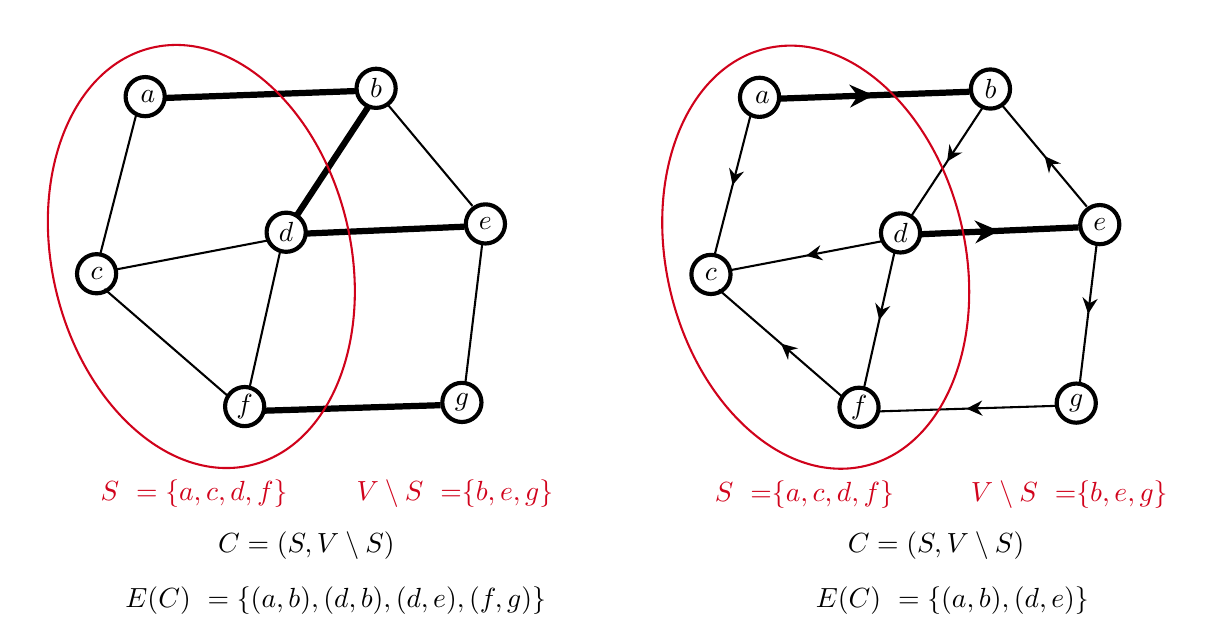
\begin{tikzpicture}[x=0.5pt,y=0.5pt,yscale=-1,xscale=1]
%uncomment if require: \path (0,445); %set diagram left start at 0, and has height of 445

%Straight Lines [id:da6859712806144006] 
\draw [color={rgb, 255:red, 0; green, 0; blue, 0 }  ,draw opacity=1 ][line width=0.75]    (282,62) -- (343,135) ;
%Straight Lines [id:da43828905709564314] 
\draw [color={rgb, 255:red, 0; green, 0; blue, 0 }  ,draw opacity=1 ][line width=2.25]    (192,283) -- (320,279) ;
%Straight Lines [id:da6385368954330931] 
\draw [color={rgb, 255:red, 0; green, 0; blue, 0 }  ,draw opacity=1 ][line width=0.75]    (77,195) -- (167,273) ;
%Straight Lines [id:da061278223687582845] 
\draw [color={rgb, 255:red, 0; green, 0; blue, 0 }  ,draw opacity=1 ][line width=0.75]    (85,181) -- (195,160) ;
%Straight Lines [id:da125058897644165] 
\draw [color={rgb, 255:red, 0; green, 0; blue, 0 }  ,draw opacity=1 ][line width=0.75]    (100,69) -- (74,170) ;
%Straight Lines [id:da7561477389708726] 
\draw [color={rgb, 255:red, 0; green, 0; blue, 0 }  ,draw opacity=1 ][line width=2.25]    (120,57) -- (258,52) ;
%Straight Lines [id:da8045438090716241] 
\draw [color={rgb, 255:red, 0; green, 0; blue, 0 }  ,draw opacity=1 ][line width=2.25]    (268,63) -- (216,142) ;
%Straight Lines [id:da7384444755679203] 
\draw [color={rgb, 255:red, 0; green, 0; blue, 0 }  ,draw opacity=1 ][line width=0.75]    (204,168) -- (182,266) ;
%Straight Lines [id:da7781378597799559] 
\draw [color={rgb, 255:red, 0; green, 0; blue, 0 }  ,draw opacity=1 ][line width=0.75]    (350,163) -- (338,262) ;
%Straight Lines [id:da6283012441188964] 
\draw [color={rgb, 255:red, 0; green, 0; blue, 0 }  ,draw opacity=1 ][line width=2.25]    (337,150) -- (222,155) ;
%Shape: Ellipse [id:dp6140347486409217] 
\draw  [color={rgb, 255:red, 208; green, 2; blue, 27 }  ,draw opacity=1 ] (182.98,322.35) .. controls (125.03,336.14) and (61.97,279.81) .. (42.15,196.51) .. controls (22.32,113.22) and (53.23,34.52) .. (111.18,20.72) .. controls (169.14,6.92) and (232.19,63.26) .. (252.02,146.55) .. controls (271.85,229.85) and (240.94,308.55) .. (182.98,322.35) -- cycle ;
%Straight Lines [id:da9976082194989311] 
\draw [color={rgb, 255:red, 0; green, 0; blue, 0 }  ,draw opacity=1 ][line width=0.75]    (726,62.5) -- (787,135.5) ;
\draw [shift={(756.5,99)}, rotate = 50.12] [fill={rgb, 255:red, 0; green, 0; blue, 0 }  ,fill opacity=1 ][line width=0.08]  [draw opacity=0] (11.61,-5.58) -- (0,0) -- (11.61,5.58) -- (7.71,0) -- cycle    ;
%Straight Lines [id:da027702952286228766] 
\draw [color={rgb, 255:red, 0; green, 0; blue, 0 }  ,draw opacity=1 ][line width=0.75]    (636,283.5) -- (764,279.5) ;
\draw [shift={(700,281.5)}, rotate = 358.21] [fill={rgb, 255:red, 0; green, 0; blue, 0 }  ,fill opacity=1 ][line width=0.08]  [draw opacity=0] (11.61,-5.58) -- (0,0) -- (11.61,5.58) -- (7.71,0) -- cycle    ;
%Straight Lines [id:da6769248424111439] 
\draw [color={rgb, 255:red, 0; green, 0; blue, 0 }  ,draw opacity=1 ][line width=0.75]    (521,195.5) -- (611,273.5) ;
\draw [shift={(566,234.5)}, rotate = 40.91] [fill={rgb, 255:red, 0; green, 0; blue, 0 }  ,fill opacity=1 ][line width=0.08]  [draw opacity=0] (11.61,-5.58) -- (0,0) -- (11.61,5.58) -- (7.71,0) -- cycle    ;
%Straight Lines [id:da10535529704419233] 
\draw [color={rgb, 255:red, 0; green, 0; blue, 0 }  ,draw opacity=1 ][line width=0.75]    (529,181.5) -- (639,160.5) ;
\draw [shift={(584,171)}, rotate = 349.19] [fill={rgb, 255:red, 0; green, 0; blue, 0 }  ,fill opacity=1 ][line width=0.08]  [draw opacity=0] (11.61,-5.58) -- (0,0) -- (11.61,5.58) -- (7.71,0) -- cycle    ;
%Straight Lines [id:da04576618929806353] 
\draw [color={rgb, 255:red, 0; green, 0; blue, 0 }  ,draw opacity=1 ][line width=0.75]    (544,69.5) -- (518,170.5) ;
\draw [shift={(531,120)}, rotate = 284.44] [fill={rgb, 255:red, 0; green, 0; blue, 0 }  ,fill opacity=1 ][line width=0.08]  [draw opacity=0] (11.61,-5.58) -- (0,0) -- (11.61,5.58) -- (7.71,0) -- cycle    ;
%Straight Lines [id:da4811530221851932] 
\draw [color={rgb, 255:red, 0; green, 0; blue, 0 }  ,draw opacity=1 ][line width=2.25]    (564,57.5) -- (702,52.5) ;
\draw [shift={(633,55)}, rotate = 537.9200000000001] [fill={rgb, 255:red, 0; green, 0; blue, 0 }  ,fill opacity=1 ][line width=0.08]  [draw opacity=0] (17.5,-8.41) -- (0,0) -- (17.5,8.41) -- (11.62,0) -- cycle    ;
%Straight Lines [id:da8150550883423667] 
\draw [color={rgb, 255:red, 0; green, 0; blue, 0 }  ,draw opacity=1 ][line width=0.75]    (712,63.5) -- (660,142.5) ;
\draw [shift={(686,103)}, rotate = 303.35] [fill={rgb, 255:red, 0; green, 0; blue, 0 }  ,fill opacity=1 ][line width=0.08]  [draw opacity=0] (11.61,-5.58) -- (0,0) -- (11.61,5.58) -- (7.71,0) -- cycle    ;
%Straight Lines [id:da45718362265354884] 
\draw [color={rgb, 255:red, 0; green, 0; blue, 0 }  ,draw opacity=1 ][line width=0.75]    (648,168.5) -- (626,266.5) ;
\draw [shift={(637,217.5)}, rotate = 282.65] [fill={rgb, 255:red, 0; green, 0; blue, 0 }  ,fill opacity=1 ][line width=0.08]  [draw opacity=0] (11.61,-5.58) -- (0,0) -- (11.61,5.58) -- (7.71,0) -- cycle    ;
%Straight Lines [id:da2742919851177712] 
\draw [color={rgb, 255:red, 0; green, 0; blue, 0 }  ,draw opacity=1 ][line width=0.75]    (794,163.5) -- (782,262.5) ;
\draw [shift={(788,213)}, rotate = 276.90999999999997] [fill={rgb, 255:red, 0; green, 0; blue, 0 }  ,fill opacity=1 ][line width=0.08]  [draw opacity=0] (11.61,-5.58) -- (0,0) -- (11.61,5.58) -- (7.71,0) -- cycle    ;
%Straight Lines [id:da49843584954749365] 
\draw [color={rgb, 255:red, 0; green, 0; blue, 0 }  ,draw opacity=1 ][line width=2.25]    (781,150.5) -- (666,155.5) ;
\draw [shift={(723.5,153)}, rotate = 177.51] [fill={rgb, 255:red, 0; green, 0; blue, 0 }  ,fill opacity=1 ][line width=0.08]  [draw opacity=0] (17.5,-8.41) -- (0,0) -- (17.5,8.41) -- (11.62,0) -- cycle    ;
%Shape: Ellipse [id:dp1685524309609875] 
\draw  [color={rgb, 255:red, 208; green, 2; blue, 27 }  ,draw opacity=1 ] (626.98,322.85) .. controls (569.03,336.64) and (505.97,280.31) .. (486.15,197.01) .. controls (466.32,113.72) and (497.23,35.02) .. (555.18,21.22) .. controls (613.14,7.42) and (676.19,63.76) .. (696.02,147.05) .. controls (715.85,230.35) and (684.94,309.05) .. (626.98,322.85) -- cycle ;

% Text Node
\draw  [line width=1.5]   (352.38, 148) circle [x radius= 14.15, y radius= 14.15]   ;
\draw (352.38,148) node   [align=left] {$\displaystyle e$};
% Text Node
\draw  [line width=1.5]   (106.48, 56) circle [x radius= 14.15, y radius= 14.15]   ;
\draw (100.98,56) node [anchor=west] [inner sep=0.75pt]   [align=left] {$\displaystyle a$};
% Text Node
\draw  [line width=1.5]   (273.38, 50) circle [x radius= 14.15, y radius= 14.15]   ;
\draw (273.38,50) node   [align=left] {$\displaystyle b$};
% Text Node
\draw  [line width=1.5]   (71.38, 184) circle [x radius= 14.15, y radius= 14.15]   ;
\draw (71.38,184) node   [align=left] {$\displaystyle c$};
% Text Node
\draw  [line width=1.5]   (208.38, 154) circle [x radius= 14.15, y radius= 14.15]   ;
\draw (208.38,154) node   [align=left] {$\displaystyle d$};
% Text Node
\draw  [line width=1.5]   (178.38, 280) circle [x radius= 14.15, y radius= 14.15]   ;
\draw (178.38,280) node   [align=left] {$\displaystyle f$};
% Text Node
\draw  [line width=1.5]   (335.38, 277) circle [x radius= 14.15, y radius= 14.15]   ;
\draw (335.38,277) node   [align=left] {$\displaystyle g$};
% Text Node
\draw (72,330.5) node [anchor=north west][inner sep=0.75pt]   [align=left] {$\displaystyle \textcolor[rgb]{0.82,0.01,0.11}{S\ =\{a,c,d,f\} \ }$};
% Text Node
\draw (257,330.5) node [anchor=north west][inner sep=0.75pt]   [align=left] {$\displaystyle \textcolor[rgb]{0.82,0.01,0.11}{V\setminus S\ =}\textcolor[rgb]{0.82,0.01,0.11}{\{b,e,g}\textcolor[rgb]{0.82,0.01,0.11}{\}}\textcolor[rgb]{0.82,0.01,0.11}{\ }$};
% Text Node
\draw (90,407.75) node [anchor=north west][inner sep=0.75pt]   [align=left] {$\displaystyle \textcolor[rgb]{0,0,0}{E( C) \ =\{( a,b) ,( d,b) ,( d,e) ,( f,g)\} \ }$};
% Text Node
\draw  [line width=1.5]   (796.38, 148.5) circle [x radius= 14.15, y radius= 14.15]   ;
\draw (796.38,148.5) node   [align=left] {$\displaystyle e$};
% Text Node
\draw  [line width=1.5]   (550.48, 56.5) circle [x radius= 14.15, y radius= 14.15]   ;
\draw (544.98,56.5) node [anchor=west] [inner sep=0.75pt]   [align=left] {$\displaystyle a$};
% Text Node
\draw  [line width=1.5]   (717.38, 50.5) circle [x radius= 14.15, y radius= 14.15]   ;
\draw (717.38,50.5) node   [align=left] {$\displaystyle b$};
% Text Node
\draw  [line width=1.5]   (515.38, 184.5) circle [x radius= 14.15, y radius= 14.15]   ;
\draw (515.38,184.5) node   [align=left] {$\displaystyle c$};
% Text Node
\draw  [line width=1.5]   (652.38, 154.5) circle [x radius= 14.15, y radius= 14.15]   ;
\draw (652.38,154.5) node   [align=left] {$\displaystyle d$};
% Text Node
\draw  [line width=1.5]   (622.38, 280.5) circle [x radius= 14.15, y radius= 14.15]   ;
\draw (622.38,280.5) node   [align=left] {$\displaystyle f$};
% Text Node
\draw  [line width=1.5]   (779.38, 277.5) circle [x radius= 14.15, y radius= 14.15]   ;
\draw (779.38,277.5) node   [align=left] {$\displaystyle g$};
% Text Node
\draw (516,331) node [anchor=north west][inner sep=0.75pt]   [align=left] {$\displaystyle \textcolor[rgb]{0.82,0.01,0.11}{S\ =}\textcolor[rgb]{0.82,0.01,0.11}{\{}\textcolor[rgb]{0.82,0.01,0.11}{a,c,d,f}\textcolor[rgb]{0.82,0.01,0.11}{\}}\textcolor[rgb]{0.82,0.01,0.11}{\ }$};
% Text Node
\draw (701,331) node [anchor=north west][inner sep=0.75pt]   [align=left] {$\displaystyle \textcolor[rgb]{0.82,0.01,0.11}{V\setminus S\ =}\textcolor[rgb]{0.82,0.01,0.11}{\{}\textcolor[rgb]{0.82,0.01,0.11}{b,e,g}\textcolor[rgb]{0.82,0.01,0.11}{\}}\textcolor[rgb]{0.82,0.01,0.11}{\ }$};
% Text Node
\draw (589,407.75) node [anchor=north west][inner sep=0.75pt]   [align=left] {$\displaystyle \textcolor[rgb]{0,0,0}{E( C) \ =\{( a,b) ,( d,e)\} \ }$};
% Text Node
\draw (157,368.5) node [anchor=north west][inner sep=0.75pt]   [align=left] {$\displaystyle C=( S,V\setminus S)$};
% Text Node
\draw (612,368.5) node [anchor=north west][inner sep=0.75pt]   [align=left] {$\displaystyle C=( S,V\setminus S)$};


\end{tikzpicture}

